\begin{pastexam}[label={px:ntu-115-bmei-alg-05}]{臺大生醫電資所 115 學年度 第 10 題}
（問答）

(8\%) Please explain steps of Kruskal's algorithm finding a minimum spanning tree. Please draw the
minimum spanning tree for the following graph.

\begin{center}
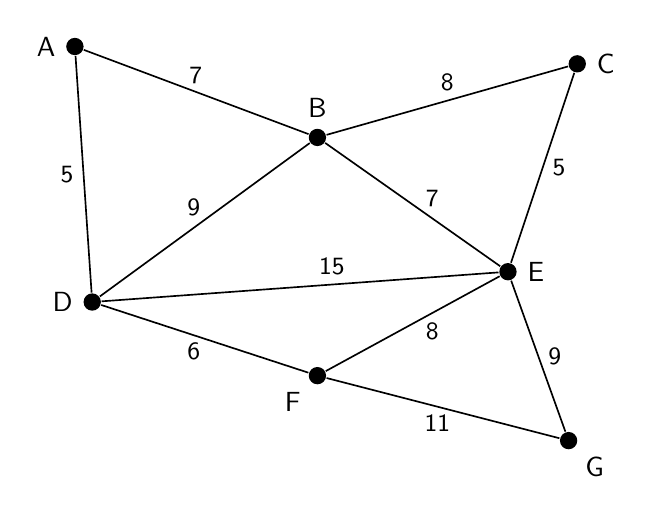
\begin{tikzpicture}[x=1.1cm,y=-1.1cm,
  v/.style={circle,fill=black,inner sep=0pt,minimum size=2.2mm},
  every node/.style={font=\sffamily\small},
  every label/.style={font=\sffamily},line width=0.6pt]
\node[v,label=left:A] (A) at (1.2,0.75) {};
\node[v,label=above:B] (B) at (4.0,1.8) {};
\node[v,label=right:C] (C) at (7.0,0.95) {};
\node[v,label=left:D] (D) at (1.4,3.7) {};
\node[v,label=right:E] (E) at (6.2,3.35) {};
\node[v,label=below left:F] (F) at (4.0,4.55) {};
\node[v,label=below right:G] (G) at (6.9,5.3) {};
\draw (A) -- node[above right=-2pt,pos=0.45] {7} (B);
\draw (B) -- node[above] {8} (C);
\draw (A) -- node[left] {5} (D);
\draw (D) -- node[above left=-2pt] {9} (B);
\draw (B) -- node[above right=-2pt,pos=0.55] {7} (E);
\draw (C) -- node[right] {5} (E);
\draw (D) -- node[above,pos=0.58] {15} (E);
\draw (F) -- node[below right=-2pt,pos=0.55] {8} (E);
\draw (D) -- node[below left=-2pt] {6} (F);
\draw (F) -- node[below left=-2pt,pos=0.55] {11} (G);
\draw (E) -- node[right] {9} (G);
\end{tikzpicture}
\end{center}
\end{pastexam}

\begin{pastsoln}
\textbf{Kruskal 演算法的步驟}（資結書第~24.2~節、虛擬碼~24.2）：
\begin{enumerate}
\item 一開始每個頂點自己是一棵樹（用互斥集合記錄哪些頂點已經連通，資結書第~13~章）。
\item 把所有邊依權重由小到大排序。
\item 依序看每一條邊 $(u, v)$：若 $u$、$v$ 屬於不同的樹（\proc{Find-Set}$(u) \ne$ \proc{Find-Set}$(v)$），
選這條邊並把兩棵樹合併（\proc{Union}）；若已經在同一棵樹，加進來會形成環，略過。
\item 選滿 $n - 1$ 條邊（$n$ 是頂點數）就停止，選到的邊就是最小生成樹。
\end{enumerate}
正確的理由是切割性質（資結書定理~24.1）：每次選的邊是連接「兩棵不同的樹」的邊裡最輕的，一定屬於某
一棵最小生成樹。 時間是排序的 $O(E \lg E)$ 加上互斥集合操作 $O(E\,\alpha(V))$，共 $O(E \lg E)$。

\textbf{本題}。 $7$ 個頂點，要選 $6$ 條邊。 十一條邊由小到大（同權重照端點字母順序）：
A--D $5$、C--E $5$、D--F $6$、A--B $7$、B--E $7$、B--C $8$、E--F $8$、B--D $9$、E--G $9$、F--G $11$、D--E $15$。
\begin{center}
\small
\begin{tabular}{rcrll}
\toprule
步 & 邊 & 權重 & 結果 & 選邊後的樹 \\
\midrule
1 & A--D & 5 & 選 & $\{A, D\}$ \\
2 & C--E & 5 & 選 & $\{A, D\}$、$\{C, E\}$ \\
3 & D--F & 6 & 選 & $\{A, D, F\}$、$\{C, E\}$ \\
4 & A--B & 7 & 選 & $\{A, B, D, F\}$、$\{C, E\}$ \\
5 & B--E & 7 & 選 & $\{A, B, C, D, E, F\}$ \\
6 & B--C & 8 & 略過：B、C 已連通（B--E--C） & 同上 \\
7 & E--F & 8 & 略過：E、F 已連通（E--B--A--D--F） & 同上 \\
8 & B--D & 9 & 略過：B、D 已連通（B--A--D） & 同上 \\
9 & E--G & 9 & 選，已滿 $6$ 條，停止 & $\{A, B, C, D, E, F, G\}$ \\
\bottomrule
\end{tabular}
\end{center}
最小生成樹的邊是 A--D、C--E、D--F、A--B、B--E、E--G，總權重 $5 + 5 + 6 + 7 + 7 + 9 = 39$。 下圖粗線是
選到的邊，細虛線是沒選的邊：
\begin{center}
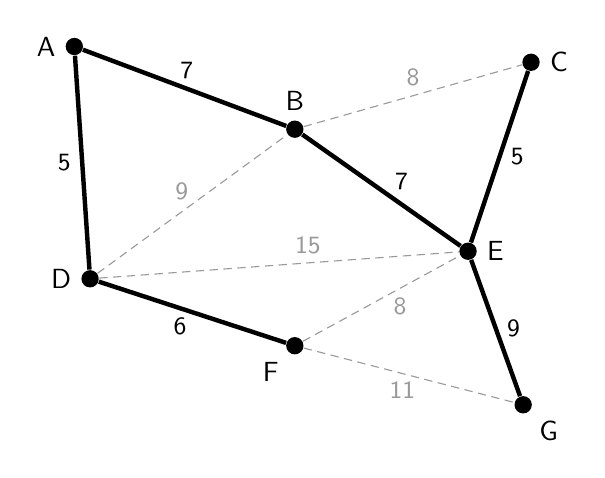
\begin{tikzpicture}[x=1.0cm,y=-1.0cm,
  v/.style={circle,fill=black,inner sep=0pt,minimum size=2.2mm},
  every node/.style={font=\sffamily\small},
  every label/.style={font=\sffamily},
  t/.style={line width=1.6pt}, n/.style={densely dashed,black!40}]
\node[v,label=left:A] (A) at (1.2,0.75) {};
\node[v,label=above:B] (B) at (4.0,1.8) {};
\node[v,label=right:C] (C) at (7.0,0.95) {};
\node[v,label=left:D] (D) at (1.4,3.7) {};
\node[v,label=right:E] (E) at (6.2,3.35) {};
\node[v,label=below left:F] (F) at (4.0,4.55) {};
\node[v,label=below right:G] (G) at (6.9,5.3) {};
\draw[t] (A) -- node[above right=-2pt,pos=0.45] {7} (B);
\draw[n] (B) -- node[above] {8} (C);
\draw[t] (A) -- node[left] {5} (D);
\draw[n] (D) -- node[above left=-2pt] {9} (B);
\draw[t] (B) -- node[above right=-2pt,pos=0.55] {7} (E);
\draw[t] (C) -- node[right] {5} (E);
\draw[n] (D) -- node[above,pos=0.58] {15} (E);
\draw[n] (F) -- node[below right=-2pt,pos=0.55] {8} (E);
\draw[t] (D) -- node[below left=-2pt] {6} (F);
\draw[n] (F) -- node[below left=-2pt,pos=0.55] {11} (G);
\draw[t] (E) -- node[right] {9} (G);
\end{tikzpicture}
\end{center}
兩組同權重的邊（兩條 $5$、兩條 $7$）都被選，兩條 $8$ 都被略過，處理順序不影響結果；B--D 和 E--G 同為 $9$，
不論誰先看，B--D 都會成環被略過、E--G 都會被選。 所以這張圖的最小生成樹是唯一的。
\end{pastsoln}
